\documentclass[../IoMusT.tex]{subfiles}
\begin{document}
\subsection{Placa de dezvoltare RaspberryPi}
\subsubsection{Prezentare generală}
Când vine vorba despre un calculator, mulți dintre noi se gândesc la PC-uri clasice sau la laptopuri. Cu toate că aceste dispozitive fac o treabă excelentă în rezolvarea task-urilor, nu sunt o alegere bună dacă vrem să lucrăm cu senzori pentru a culege date sau dorim să punem în funcțiune niște actuatori pe baza datelor colectate. Pentru astfel de operațiuni, și nu numai, ai fost create plăcile de dezvoltare sau SBC \footnote{Single-board computer}. Un astfel de calculator este și Rasbperry Pi-ul care a fost creat în Marea Britanie cu scopul de a promova predarea informaticii în școlile și țările în curs de dezvoltare \cite{SBC} dar poate fi utilizat pentru o varietate de scopuri precum robotica sau într-o gamă largă de aplicații în domeniul IoT. Aceste plăci, de mărimea a unui card de credit, au devenit repede populare din cauza dimensiunilor și a accesibilității în ceea ce privește prețul acestora. 
\begin{figure}[h]
\centering
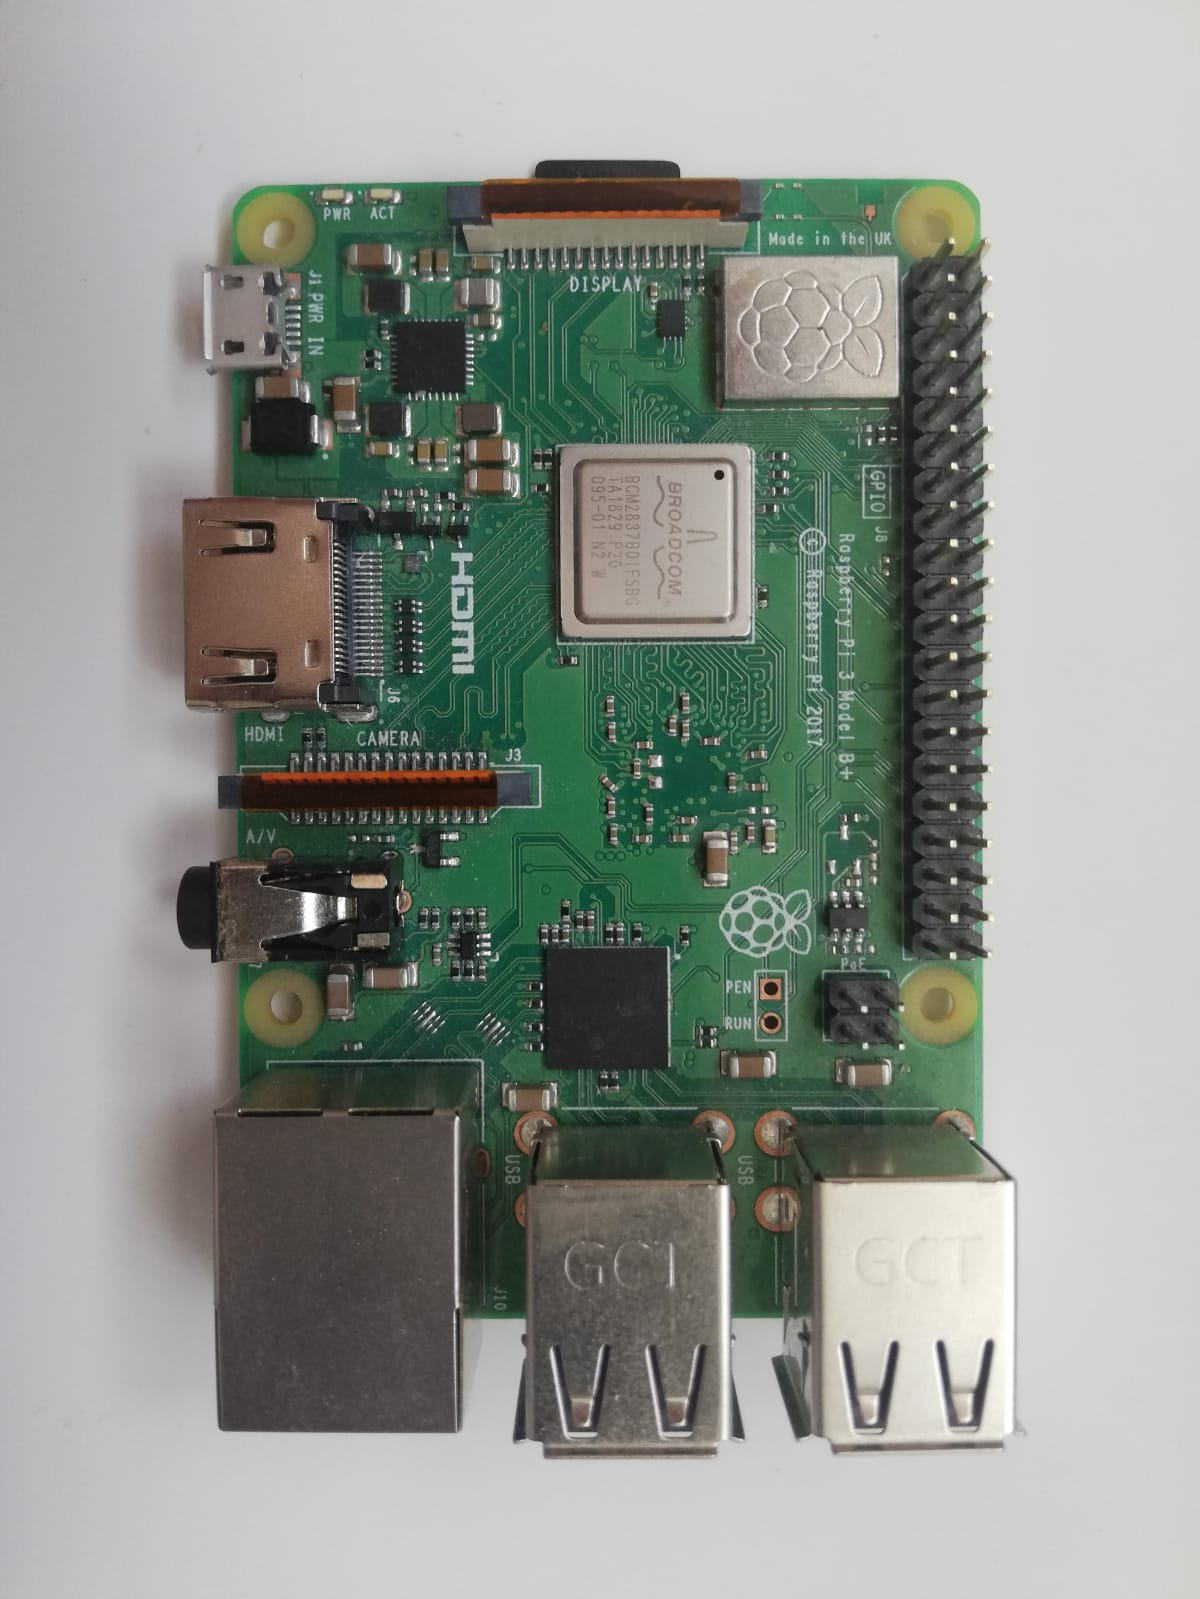
\includegraphics[scale=0.12, angle=90]{pi}
\caption{Raspberry Pi 3 model B+}
\end{figure}
\\
\par În decursul anilor s-au lansat mai multe versiuni al acestei plăci, fiecare venind cu o îmbunătățire pe partea de software sau hardware. Pentru realizarea acestui proiect eu am folosit un Raspberry Pi 3 model B+ care, din punctul meu de vedere, este un model perfect de a începe a lucra la proiecte IoT. Datorită faptului că este un single-board computer, componentele sale sunt plasate într-un singur circuit imprimat. Acest circuit sprijină mecanic și conectează electric componenetele electrice folosind piste conductoare. În cazul acestei plăci printre componentele atașate pe circuit se poate enumăra microprocesorul, memoria RAM \footnote{Random access memory}, diferitele porturi de intrare și ieșire sau pinurile GPIO \footnote{General-purpose input/ouput}.
\\
\par
\subsubsection{Folosirea pinurilor}
Pe fiecare model de placă RaspberryPi se pot observa de-a lungul marginii  superioare pinii GPIO. Pe plăcile curent se află 40 de astfel de pini, fiecare putănd fi programat ca un pin de intrare sau ieșire având astfel șansa de a le utiliza într-o gamă largă de scopuri.
\\
\par Există câte două pinuri cu un voltaj de 5, respectiv 3.3 și opt pini la sol care nu pot fi configurate. Celelalte sunt pinuri generale de 3V3 asta înseamnând că la ieșire sunt setate la 3V3 și la intrare sunt tolerate la 3V3 \cite{RaspPi}. O caracteristică importantă a acestori pini generali este modularea lățimii pulsurilor (PWM\footnote{Pulse Width Modulation}) cu ajutorul căruia putem controla dispozitivele analogice cu o ieșire digitală \cite{PWM} find o metodă alternativă de control armonic. 
\\
\par Fiecare pin în parte (înafară de cele de ground, de 3V3 și 5V) au un număr specific care vine în ajutor în momentul programării acestora. Există două sisteme de numerotare: sistemul Broadcom (care este folosit cel mai des) și numerotarea fizică a pinurilor. Cele mai multe biblioteci din Python folosesc sistemul Broadcom așa câ și în proiectul de față s-a folosit tot acest sistem de numărotare.

\subsubsection{Conectarea la internet}
%exista mai multe programe cautare ip....???
Conectarea plăcii Raspberry Pi la internet se poate face în două feluri: prin cablu de internet, placa având port de internet, sau prin WIFI. În abele cazuri dacă vrem să accesăm linia de comandă a plăcii respective, conectarea se face prin prin SSH\footnote{Secure Shell}, pentru care trebuie aflată adresa IP. Acest lucru se poate face în mai multe feluri, existând mai multe programe de căutare a adreselor. Datorită faptului că adresa IP dinamică se schimbă mereu, după cum sugerează și numele, pentru a putea lucra mai ușor și eficient cu placa de dezvoltare Raspberry Pi s-a folosit o adresă IP statică. Astfel de fiecare dată când dorim să ne conectăm la ea, fie prin socket-uri sau prin alte metode, adresa va rămâne aceași. Se poate seta o adresă statică atât pentru conectarea la internet prin cablu cât și prin WIFI.

\subsubsection{Conectarea plăcii la instrumente muzicale}
Conectarea unei plăci Raspberry Pi la un instrument muzical se face cu ajutorul unui cablu MIDI USB. Pentru a fi posibilă această operațiune instrumentul respectiv trebuie să fie electric și să suporte interfață digitală. Partea USB a cablului respectiv se va conecta la unul dintre porturile plăcii de dezvoltare iar cealaltă parte se va conecta la porturile MIDI ale instrumentului respectiv. Partea conectată la pian a cablului se termină în mai multe conectoare DIN \footnote{Deutsches Institut für Normung} cu cinci pini de 180\si{\degree}.
\begin{figure}[h]
\centering
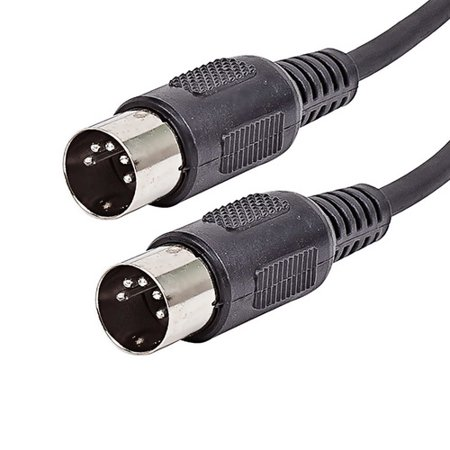
\includegraphics[scale=0.35]{midi}
\caption{Mufă MIDI}
\label{fig:midi}
\end{figure}  
 Un singur concetor ar transporta  mesajele doar într-o singură direcție, deci pentru a avea o comunicare în două sensuri avem nevoie de cel puțin două astfel de conectori (vezi figura \ref{fig:midi}). Pentru că majoritatea instrumentelor nu copiază mesajele în porturile de ieșire, există și varinate de cablu care au trei mufe, al treilea fiind cel de THRU care este destinat pentru transmiterea datelor către un alt instrument. În cazul nostru sunt deajunse concetorii de IN și OUT. Însă trebuie avut grijă pentru că etichetarea acestor mufe ca fiind IN și OUT ne poate duce în eroare când vine vorba despre conectare pentru că acestea nu vor funcționa dacă sunt conectate la aceleași porturi MIDI etichetate pe un instrument electric. Acest lucru se datoriează faptului că fluxul de date indicat pe mufe arată direcția  în care datele vor curge către calculator, nu portul  de pe instrument la care  trebuie conectat fiecare cablu \cite{Midi}. Deci mufa IN se va conecta la portul OUT și mufa OUT la cel de IN.

\subsection{Actuatori folosiți pentru realizarea hapticii}
\subsubsection{Motoare de vibrați LRA}
Motoarele de vibrații pot fi de mai mult tipuri astfel alegerea unui tip de motor depinde în cea mai mare parte de cerințe, de unde și pentru ce va fi folosit. Există două mari categorii de astfel de motoare și anume ERM și LRA. Diferența dintre acestea, înafară de mărimea lor, este modul în care funcționează. Primul tip de motor folosește o masă mică dezechilibrată pe un motor cu curent continuu atunci când se rotește creând o forță care se traduce prin vibrații. Servomotoarele rezonante liniare (LRA) conțin o masă internă mică atașată la un arc, care creează o forță atunci când sunt conduse de curent \cite{LRA}. În tehnologiile unde e prezent feedback-ul haptic, de cele mai multe ori se folosesc motoare de tip LRA din cazua mărimii și a faptului că modularea amplitudinii este foarte ușoară. În realizarea acestui proiect s-au folosit mai multe motoare de vibrații de acest tip pentru obținerea vibrațiilor de intensitate dorită.
\\
\par Modul în care aceste motore sunt puse în funcțiune este prin conectarea firelor la pinurile corespunzătoare de pe placa Raspberry Pi. Cu ajutorul PWM putem controla atât valoarea la care aceste motoare vor vibra încât și frecvența acestora.
\begin{figure}[h]
\centering
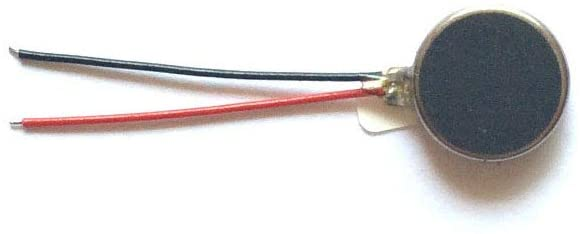
\includegraphics[scale=0.2, angle=90]{LRA}
\caption{Motor de vibrații LRA}
\end{figure}
Modelul folosit de mine are firele de culoare negru și roșu, dar sunt și motoare care merg pe varianta de roșu și albastru. Scopul principal a acestor culori este de a ști la ce pini trebuie conectați: culoarea roșie se conectează la un pin GPIO iar cea neagră la pământ (ground pin).
\end{document}